\section{Il progetto di un sistema di controllo in retrazione - Parte 3}

\subsection{Sistemi di controllo per la regolazione}

\begin{figure}[h!]
  \centering
  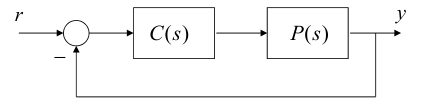
\includegraphics[width=0.8\textwidth]{./images/lez16_controllo.png}
  \caption{Schema di controllo}
  \label{fig:lez16_controllo}
\end{figure}


Assumendo che $P(s)$ sia definita come:
\begin{equation}
  P(s) = \frac{b(s)}{a(s)} = \frac{b_{n-1}^{n-1} + \dots + b_0}{s^n + a_{n-1}s^{n-1} + \dots + a_0}
\end{equation}

con $b(s)$ e $a(s)$ coprimi.

Il problema di regolazione (asintotica) ha soluzione se e solo se $P(0) \neq
0$.


\subsection{I regolatori PID}

Tenendo l'immagine \ref{fig:lez16_controllo}:
\begin{equation}
  C(s) = K_p(1 + T_d s + \frac{1}{T_i s})
\end{equation}
Dove:
\begin{itemize}
  \item $K_p$ costante proporzionale
  \item $T_d$ costante di tempo dell'azione derivativa
  \item $T_i$ costante di tempo dell'azione integrale
  \item $\frac{1}{K_p}$ banda proporzionale
\end{itemize}


\subsection{Progetto frequenziale del regolatore PID}


Considerando che la risposta armonica è definita come:
\begin{equation}
  C(j\omega) = K_p(1 + j\omega T_d + \frac{1}{j\omega T_i})
\end{equation}

Una proprietà specifica $\omega_n := \frac{1}{\sqrt{T_d T_i}}$, segue che 
$C(j\omega_n) = K_p$.

% \subsection{Implementazione dei regolatori PID}
% \subsubsection{Limitazione dell'azione derivativa}
%
% Si impone:
% \begin{equation}
%   \tau = \frac{T_d}{N}, \quad N = 5 \div 20
% \end{equation}
%
% \subsubsection{Desaturazione dell'azione integrale}
%
%



\subsection{Conclusioni}
Le tecniche utili alla sintesi di un controllo in retroazione a struttura
prefissata sono:
\begin{itemize}
  \item Criterio e tabella di Routh
  \item Diagramma di Nyquist
  \item Diagramma di Bode
  \item Cancellazione polo-zero
  \item Metodo del polinomio caratteristico
  \item Metodo del luogo delle radici
\end{itemize}

